%!TEX program = xelatex

\documentclass{progartcn}
\usepackage{graphicx}
\usepackage[dvipsnames]{xcolor}
\usepackage{wrapfig}
\usepackage{enumerate}
\usepackage{amsmath,mathrsfs,amsfonts}
\usepackage{booktabs}
\usepackage{tabularx}
\usepackage{colortbl}
\usepackage{multirow,makecell}
\usepackage{multicol}
\usepackage{ulem} % \uline
\usepackage{listings}
\usepackage{tikz}
\usepackage{tcolorbox}
\usepackage{fontawesome}


\title{\bfseries\sffamily
  计算机系统结构实验4 \\ 简单的类 MIPS 单周期处理器功能部件的设计与实现(二)
}
\author{胡晨志 521021910107}
\date{}


\begin{document}

\sloppy % 解决中英文混排文字超出边界问题


\maketitle
\thispagestyle{empty}

\begin{abstract}
\noindent 在lab04中,我继续学习Verilog语言并实现了寄存器、数据存储器和有符号扩展单元等功能,为后续搭建单周期处理器和流水线作准备。

\vspace{2ex}
\noindent \textbf{关键字:}Vivado,\hspace{.5em}Verilog
\end{abstract}

\tableofcontents

\setcounter{page}{0}
\newpage

\section{实验目的}

\begin{itemize}
  \item 理解寄存器、数据存储器、有符号扩张单元的IO定义
  \item Register 的设计实现
  \item Data Memory 的设计实现
  \item 有符号扩展部件的实现
  \item 有符号扩展部件的实现
  \item 对功能模块进行仿真
\end{itemize}

\section{原理分析}

\subsection{Vivado 工程的基本组成}

Vivado 工程的基本组成如下:

\begin{itemize}
  \item design source .v 文件:\verb|dataMemory.v|,\verb|Registers.v|,\verb|signext.v|
  \item simulation source .v 文件:\verb|Datamemory_tb.v|,\verb|Registers_tb.v|,\verb|signext_tb.v|
\end{itemize}

\subsection{实现原理}

按照实验指导书上各个部件的端口创建模块。统一通过时钟下降沿来同步写数据操作。注意Register写数据后要改变输出端口的值。

\section{功能实现}

基于上述即可完成主控制模块的功能。三个模块的代码分别如 </>CODE \ref{cd:1},</>CODE \ref{cd:2},</>CODE \ref{cd:3} 所示。

\begin{lstlisting}[language=verilog,caption={dataMemory.v},label={cd:1}]
`timescale 1ns / 1ps 

module dataMemory(
    input Clk,
    input [31:0] address,
    input [31:0] writeData,
    input memWrite,
    input memRead,
    output [31:0] readData
    );
    
    reg [31:0] memFile[0:63];
    reg [31:0] readdata;
    integer i;
    
    initial begin
        for (i = 0; i < 64; i = i + 1)
            memFile[i] = 0;
    end
    
    always@ (memRead or memWrite or address)
        begin
            if (memWrite ==1)
                readdata = 0;
            else if (memRead == 1)
                readdata = memFile[address];
            else readdata = 0;
        end
    always@ (negedge Clk)
        begin
            if (memWrite == 1)
                memFile[address] = writeData;
        end
    assign readData = readdata;
endmodule
\end{lstlisting}

\begin{lstlisting}[language=verilog,caption={Registers.v},label={cd:2}]
`timescale 1ns / 1ps
module Registers(
    input Clk,
    input [25:21] readReg1,
    input [20:16] readReg2,
    input [4:0] writeReg,
    input [31:0] writeData,
    input regWrite,
    output [31:0] readData1,
    output [31:0] readData2
    );
    
    reg [31:0] regFile[31:0];
    reg [31:0] readdata1;
    reg [31:0] readdata2;
    integer i;

    initial begin
        for (i = 0; i < 32; i = i + 1)
            regFile[i] = 0;
    end
    
    always @(readReg1 or readReg2 or writeReg)
        begin
            readdata1 = regFile[readReg1];
            readdata2 = regFile[readReg2];
        end
    
    always @(negedge Clk)
        begin
            if (regWrite)
                begin
                    regFile[writeReg] = writeData;
                    if (writeReg == readReg1)
                        readdata1 = regFile[readReg1];
                    if (writeReg == readReg2)
                        readdata2 = regFile[readReg2];
                end
        end
    assign readData1 = readdata1;
    assign readData2 = readdata2;
endmodule

\end{lstlisting}

\begin{lstlisting}[language=verilog,caption={signext.v},label={cd:3}]
`timescale 1ns / 1ps

module signext(
    input [15:0] inst,
    output [31:0] data
    );
    assign data = {{16{inst[15]}}, inst[15:0]};
endmodule
\end{lstlisting}

实现上述后,生成 \verb|Ctr_tb.v| 的激励文件用以仿真测试.

\section{结果验证}

\subsection{测试用激励文件}

按照实验指导书的要求编写 \verb|dataMemory_tb.v|,\verb|Registers_tb.v|,\verb|signext.v|文件,代码如 </>CODE \ref{cd:4}, </>CODE \ref{cd:5}, </>CODE \ref{cd:6}, 所示。

\begin{lstlisting}[language=verilog,caption={dataMemory\_tb.v},label={cd:4}]
`timescale 1ns / 1ps

module dataMemory_tb(

    );
    reg Clk;
    reg [31:0] address;
    reg [31:0] writeData;
    reg memWrite;
    reg memRead;
    wire [31:0] readData;
    
    dataMemory u0 (
        .Clk(Clk),
        .address(address),
        .writeData(writeData),
        .memWrite(memWrite),
        .memRead(memRead),
        .readData(readData)
    );
    
    parameter PERIOD = 100;
    
    always #(PERIOD) Clk = !Clk;
    
    initial begin
        Clk = 0;
        address = 0;
        writeData = 0;
        memWrite = 0;
        memRead = 0;
        
        #185;
        memWrite = 1'b1;
        address = 32'b00000000000000000000000000000111;
        writeData = 32'b11100000000000000000000000000000;
        
        #100;
        memWrite = 1'b1;
        writeData = 32'hffffffff;
        address = 32'b00000000000000000000000000000110;
        
        #185;
        memRead = 1'b1;
        address = 7;
        memWrite = 1'b0;
        
        #80;
        memWrite = 1;
        address = 8;
        writeData = 32'haaaaaaaa;
        
        #80;
        memWrite = 0;
        address = 6;
        memRead = 1;
    end
endmodule
\end{lstlisting}

\begin{lstlisting}[language=verilog,caption={Registers\_tb.v},label={cd:5}]
`timescale 1ns / 1ps

module Registers_tb(

    );
    reg Clk;
    reg [25:21] readReg1;
    reg [20:16] readReg2;
    reg [4:0] writeReg;
    reg [31:0] writeData;
    reg regWrite;
    wire [31:0] readData1;
    wire [31:0] readData2;
    
    Registers u0 (
        .Clk(Clk),
        .readReg1(readReg1),
        .readReg2(readReg2),
        .writeReg(writeReg),
        .writeData(writeData),
        .regWrite(regWrite),
        .readData1(readData1),
        .readData2(readData2)
    );
    
    parameter PERIOD = 100;
    
    always #(PERIOD) Clk = !Clk;
    
    initial begin
        // Initialize Inputs
        Clk = 1;
        readReg1 = 0;
        readReg2 = 0;
        writeReg = 0;
        writeData = 0;
        regWrite = 0;
        
        //Current Time: 285ns
        #285;
        regWrite = 1'b1;
        writeReg = 5'b10101;
        writeData = 32'b11111111111111110000000000000000;
        
        //Current Time: 485ns
        #200;
        writeReg = 5'b01010;
        writeData = 32'b00000000000000001111111111111111;
        
        #200;
        regWrite = 1'b0;
        writeReg = 5'b00000;
        writeData = 32'b00000000000000000000000000000000;
        
        //Current Time: 735ns
        #50;
        readReg1 = 5'b10101;
        readReg2 = 5'b01010;
    end
endmodule
\end{lstlisting}

\begin{lstlisting}[language=verilog,caption={signext\_tb.v},label={cd:6}]
`timescale 1ns / 1ps

module signext_tb(

    );
    reg [15:0] inst;
    wire [31:0] data;
    
    signext u0 (
        .inst(inst),
        .data(data)
    );
    
    initial begin
        inst = 16'b0000000000000000;
        
        #100;
        inst = 16'b0000000000000001;
        
        #100;
        inst = 16'b1111111111111111;
        
        #100;
        inst = 16'b0000000000000010;
        
        #100;
        inst = 16'b1111111111111110;
    end
endmodule
\end{lstlisting}

\subsection{仿真测试}

数据存储器、寄存器和有符号扩展单元仿真结果分别如图\ref{fig:1},\ref{fig:2},\ref{fig:3}所示。

\begin{figure}[htbp]
    %是可选项 h表示的是here在这里插入,t表示的是在页面的顶部插入
    \centering
    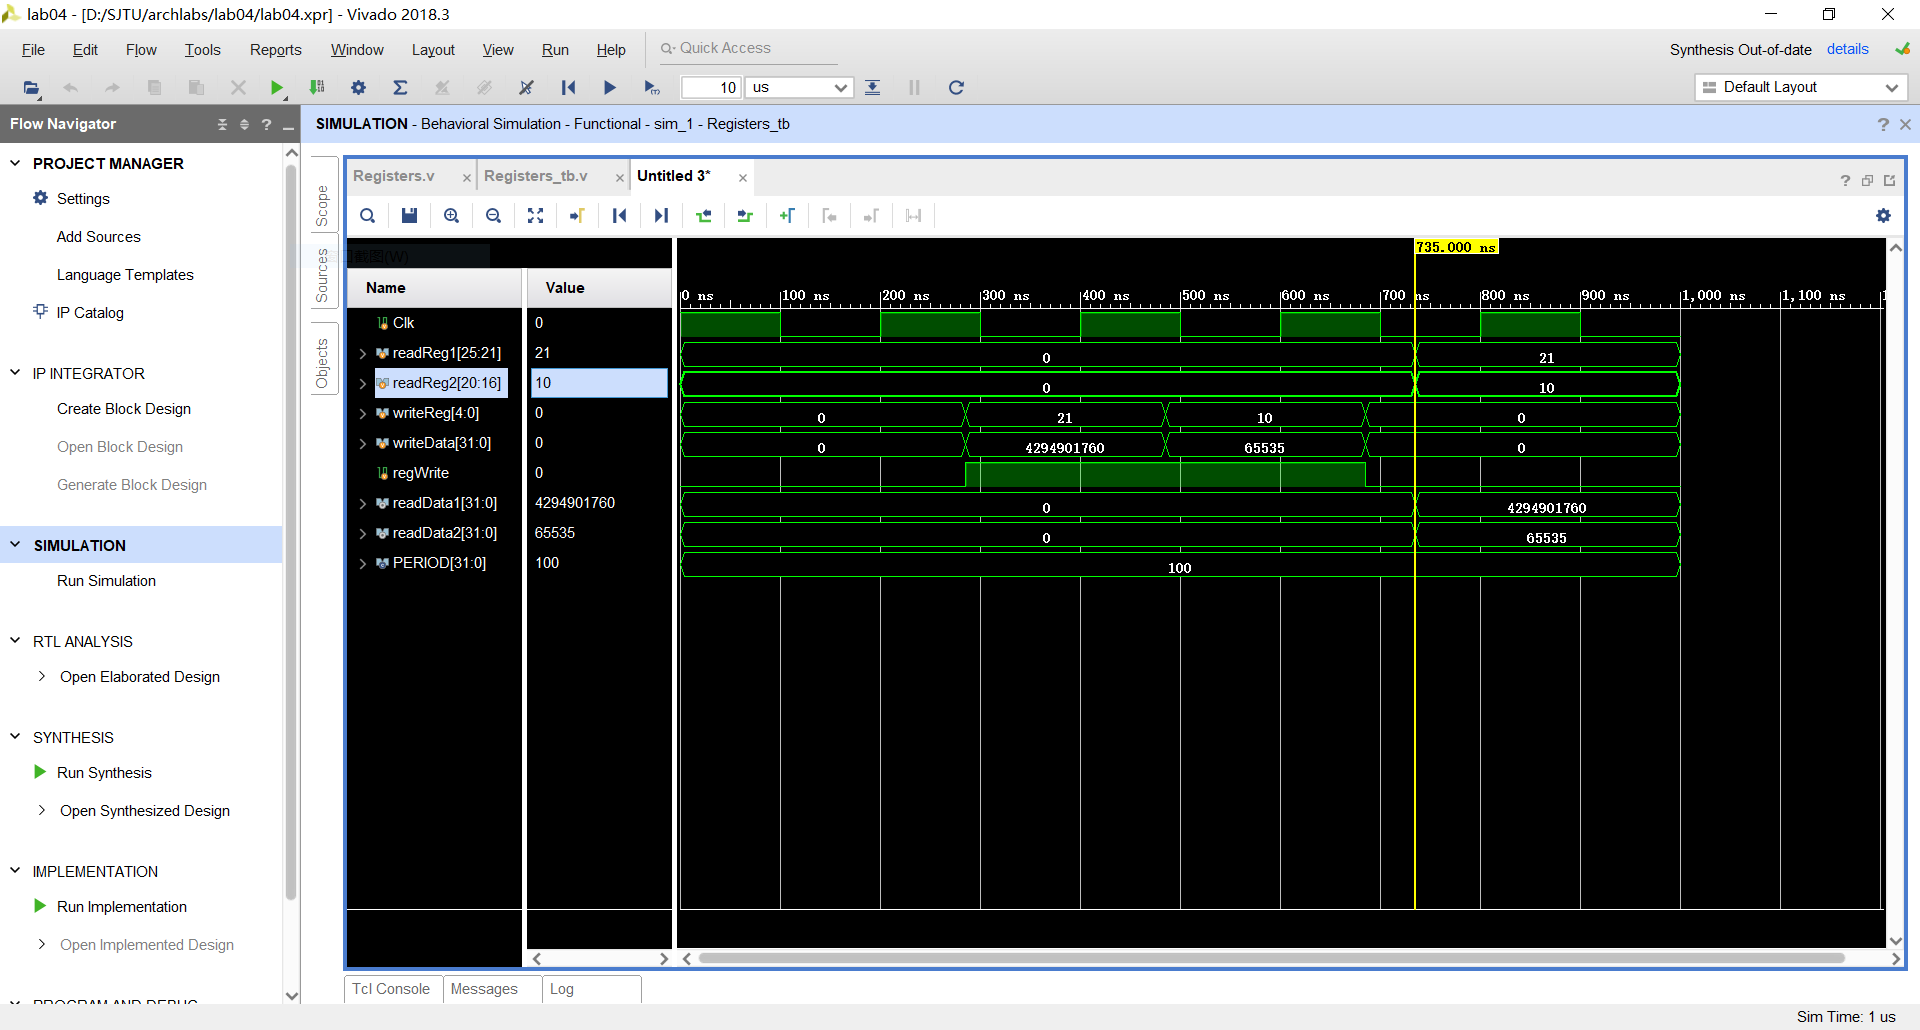
\includegraphics[scale=0.3]{../figure/04/lab04-1.PNG}
    \caption{数据存储器实验结果}\label{fig:1}
\end{figure}

\begin{figure}[htbp]
    %是可选项 h表示的是here在这里插入,t表示的是在页面的顶部插入
    \centering
    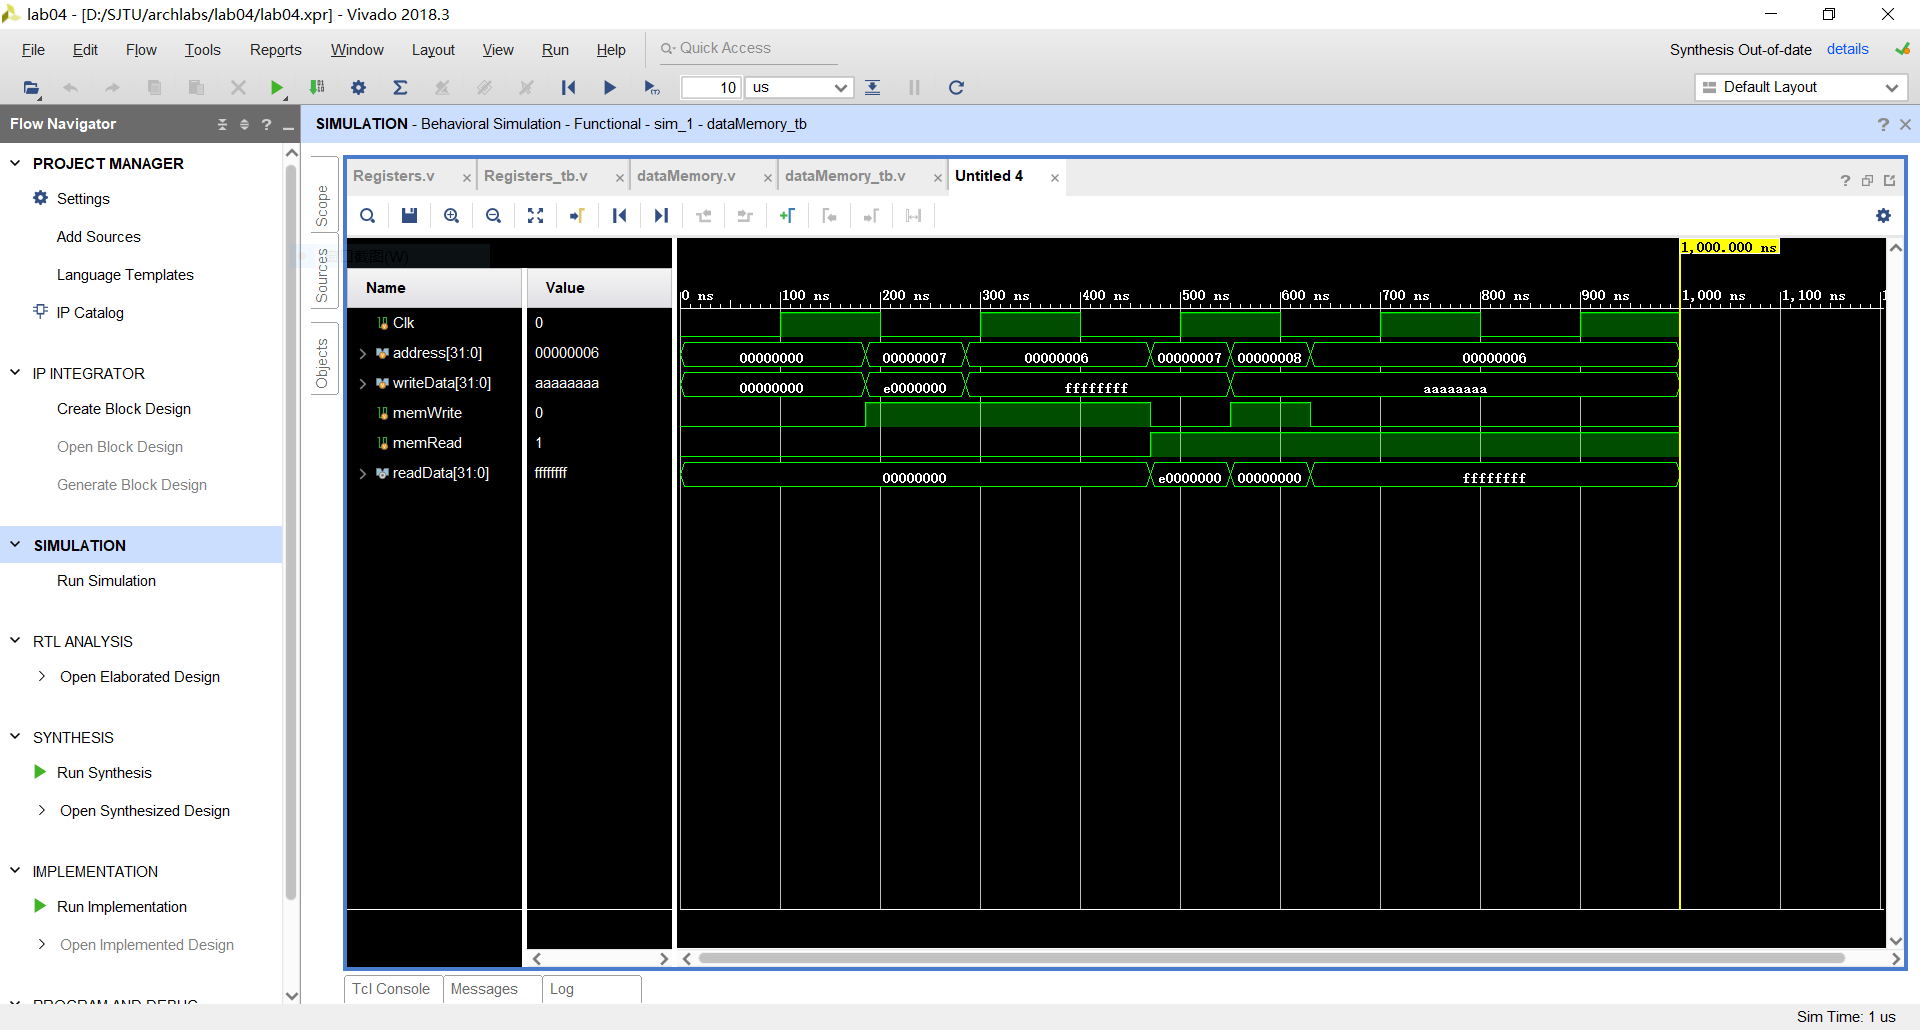
\includegraphics[scale=0.3]{../figure/04/lab04-2.PNG}
    \caption{寄存器实验结果}\label{fig:2}
\end{figure}

\begin{figure}[htbp]
    %是可选项 h表示的是here在这里插入,t表示的是在页面的顶部插入
    \centering
    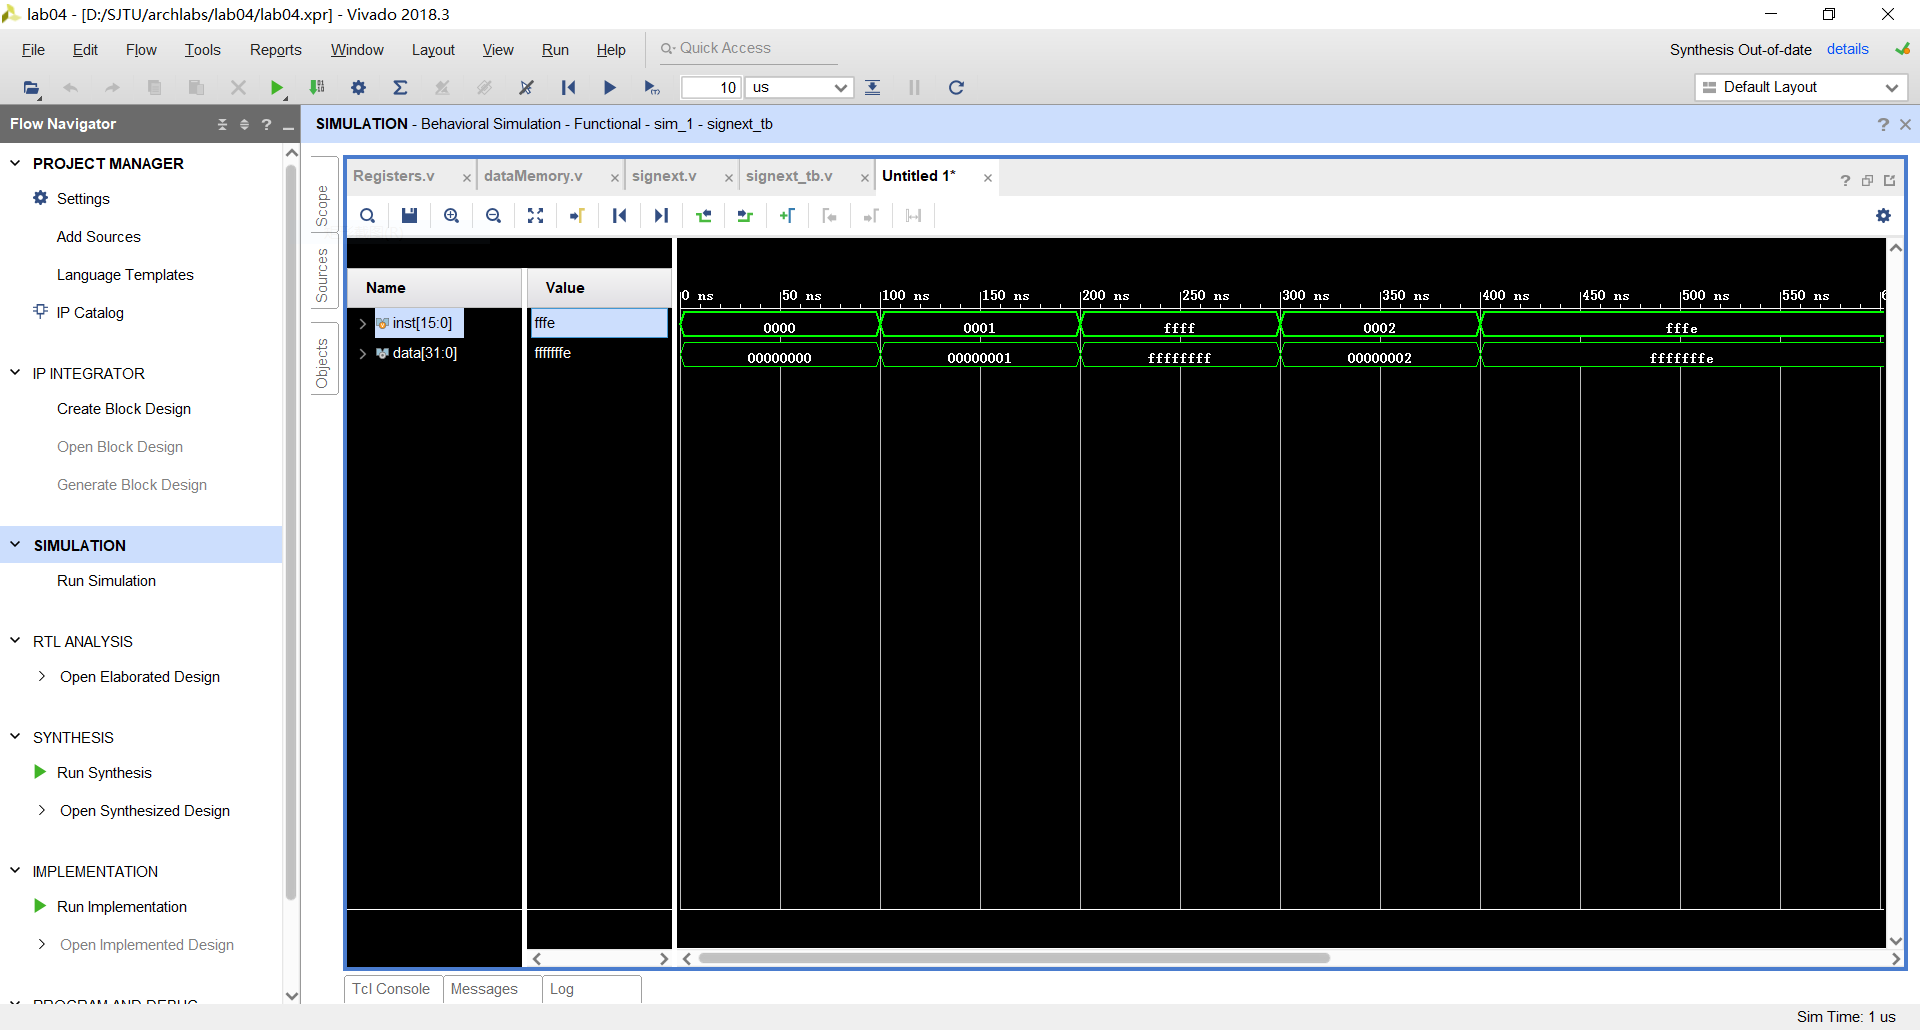
\includegraphics[scale=0.3]{../figure/04/lab04-3.PNG}
    \caption{有符号扩展单元实验结果}\label{fig:3}
\end{figure}


\section{反思与总结}

本次实验的主要难点在于写数据操作的同步问题,具体实现时通过时钟下降沿进行同步。此处统一使用下降沿也是为了方便后续实验。

在编写有符号扩展扩展单元时刚开始我的写法十分笨拙,先判断高位是一还是零,然后用if语句分别进行扩展。在老师的指导下我修改成了现在这个比较简单的版本。

\end{document}
